\providecommand{\main}{..}
\documentclass[\main/thesis.tex]{subfiles}

\begin{document}
\begin{appendices}
\chapter*{Appendix}

An extension of the feature importance utilization figures shown in Section~\ref{ssec:xgb_aenc_embd_feat_importances} is displayed in Figure~\ref{fig:xgb_aenc_top_1000_features_labelwise_count} and Figure~\ref{fig:xgb_aenc_top_100_features_labelwise_count}.


\begin{figure}[t]
    \centering
    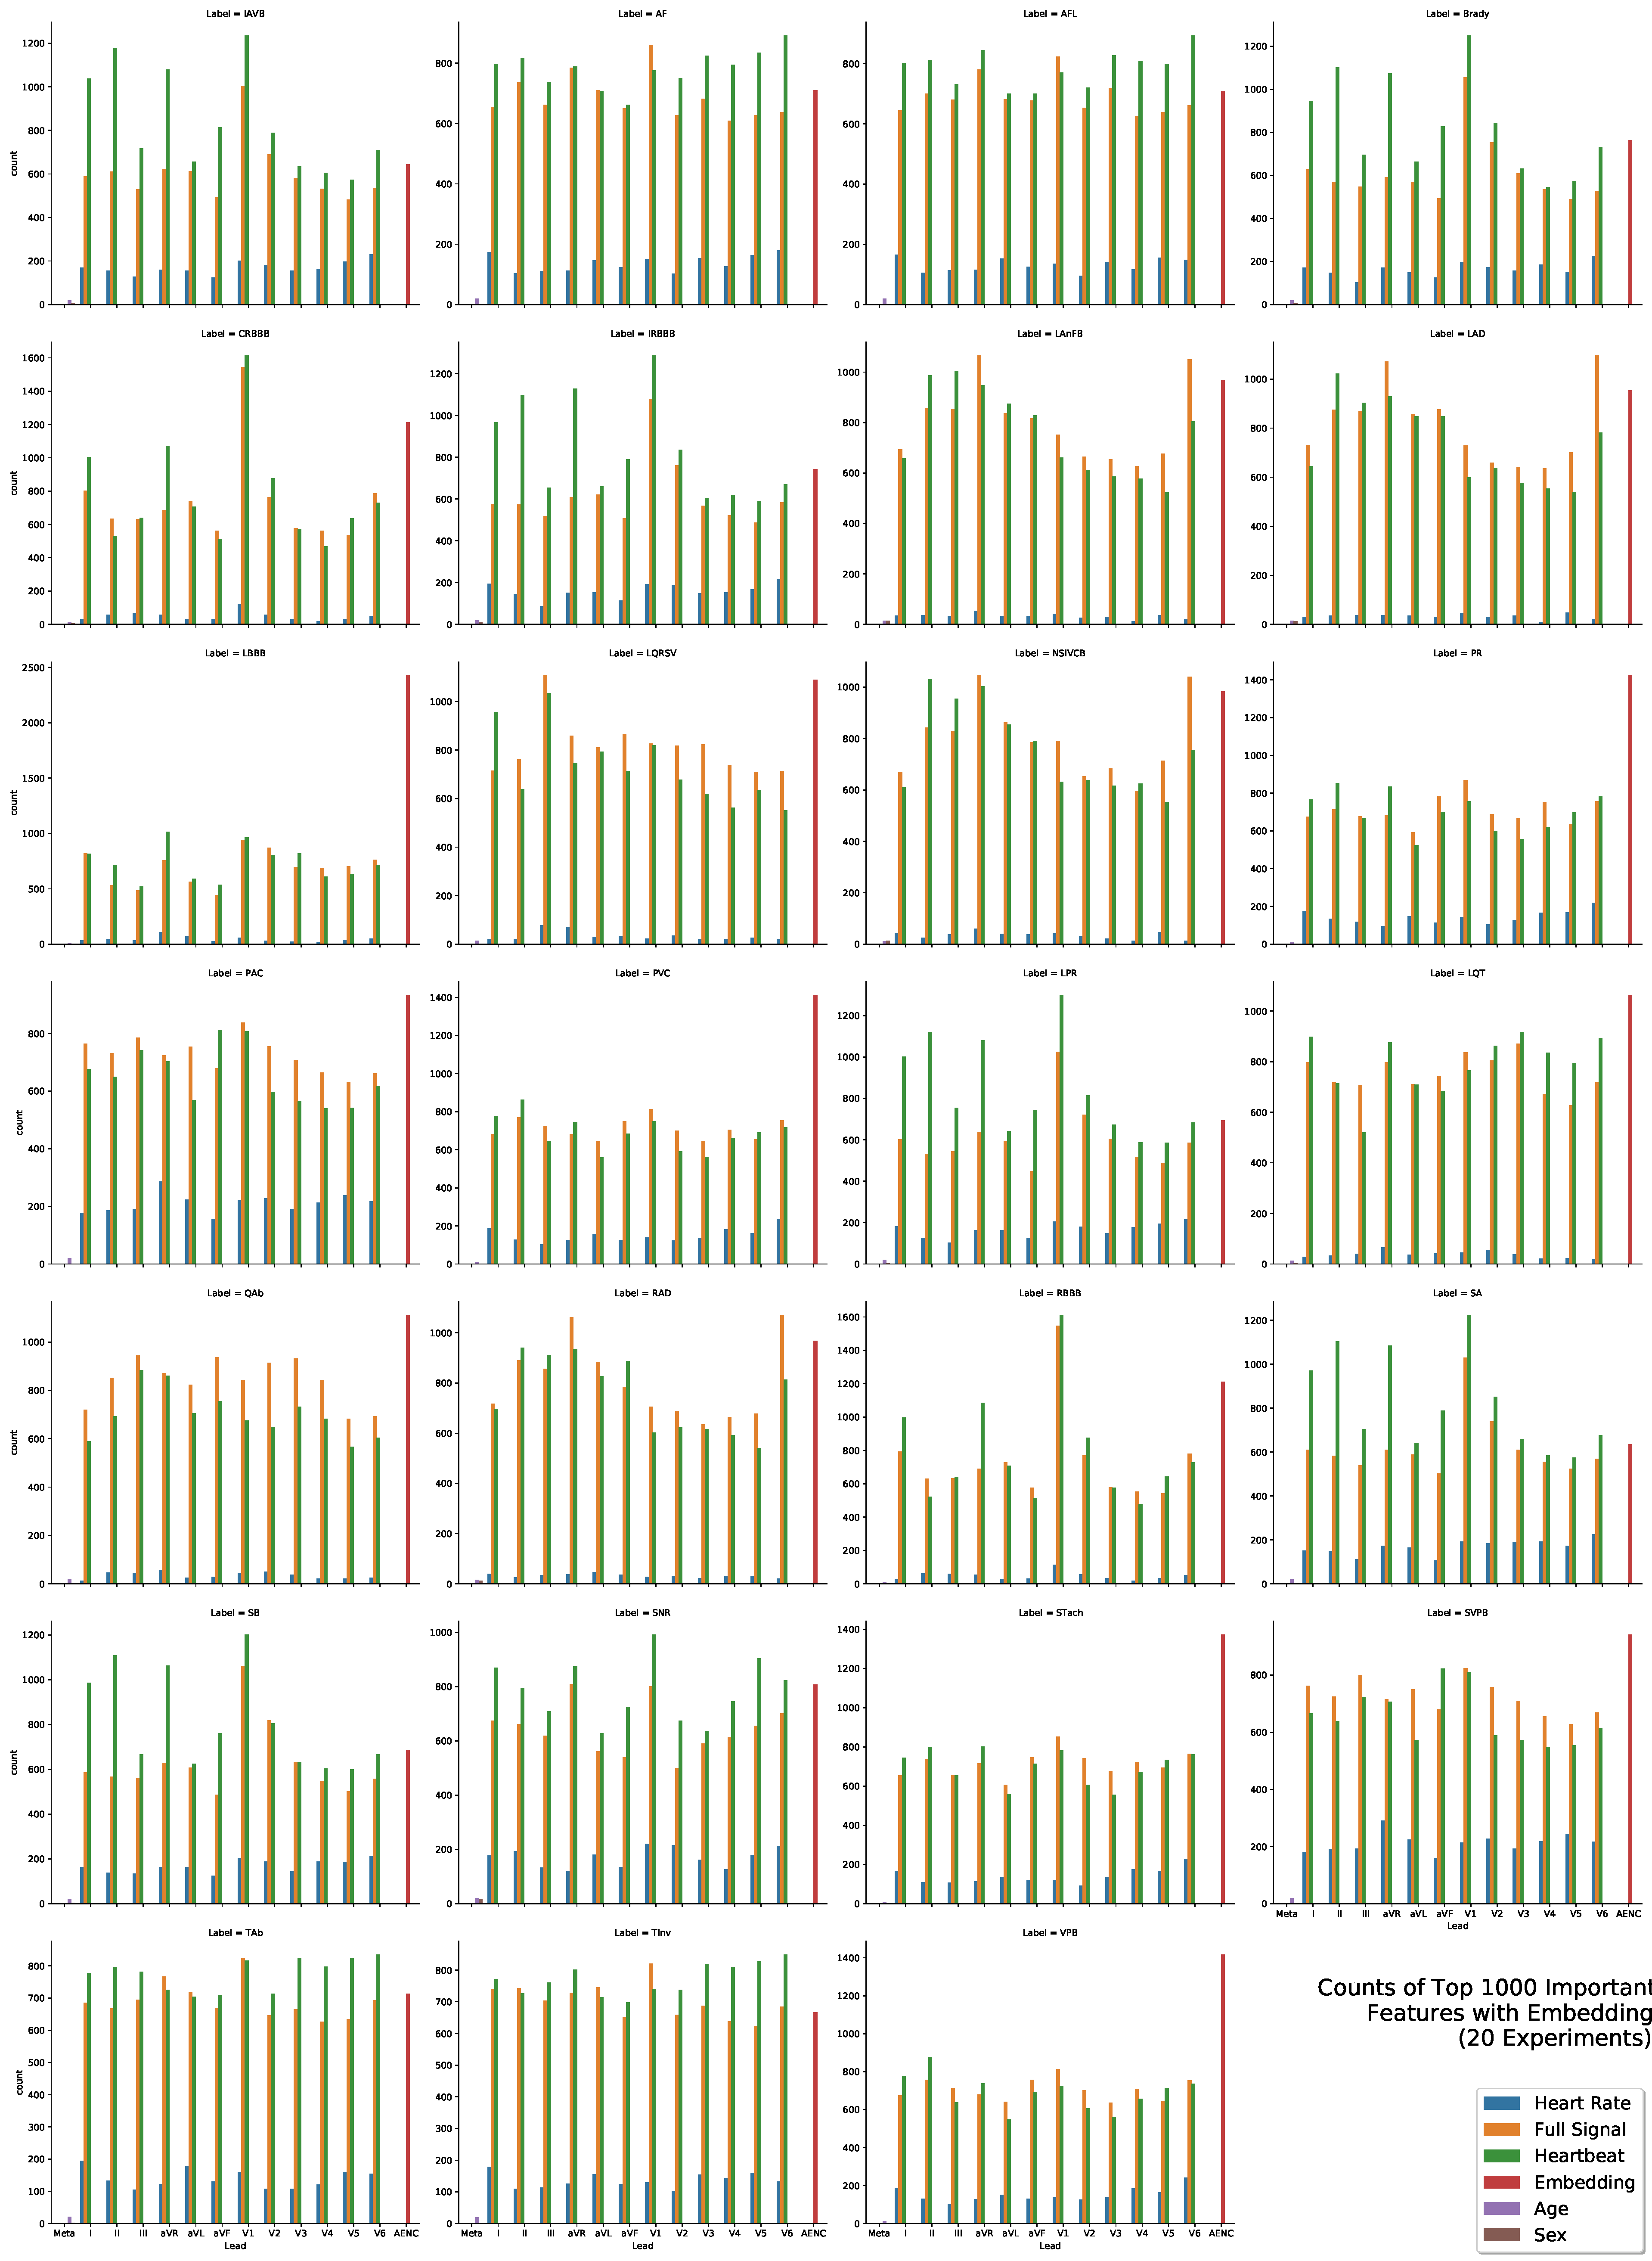
\includegraphics[width=\textwidth]{figure/top_1000_feature_importances_all_w_embedding.pdf}
    \caption{Feature importances summary of Configuration~\ref{item:xgb_aenc_model_top_1000_w_embd}: ``Top 1000 Features with Embeddings", aggregated count over 20 independent experiments. Each of the 27 diagnosed labels displayed separately, showcasing feature derived lead (alternatively Meta or Autoencoder), and category (heart rate, full waveform signal, heartbeat, embedding, age, sex).}
    \label{fig:xgb_aenc_top_1000_features_labelwise_count}
\end{figure}

\begin{figure}[t]
    \centering
    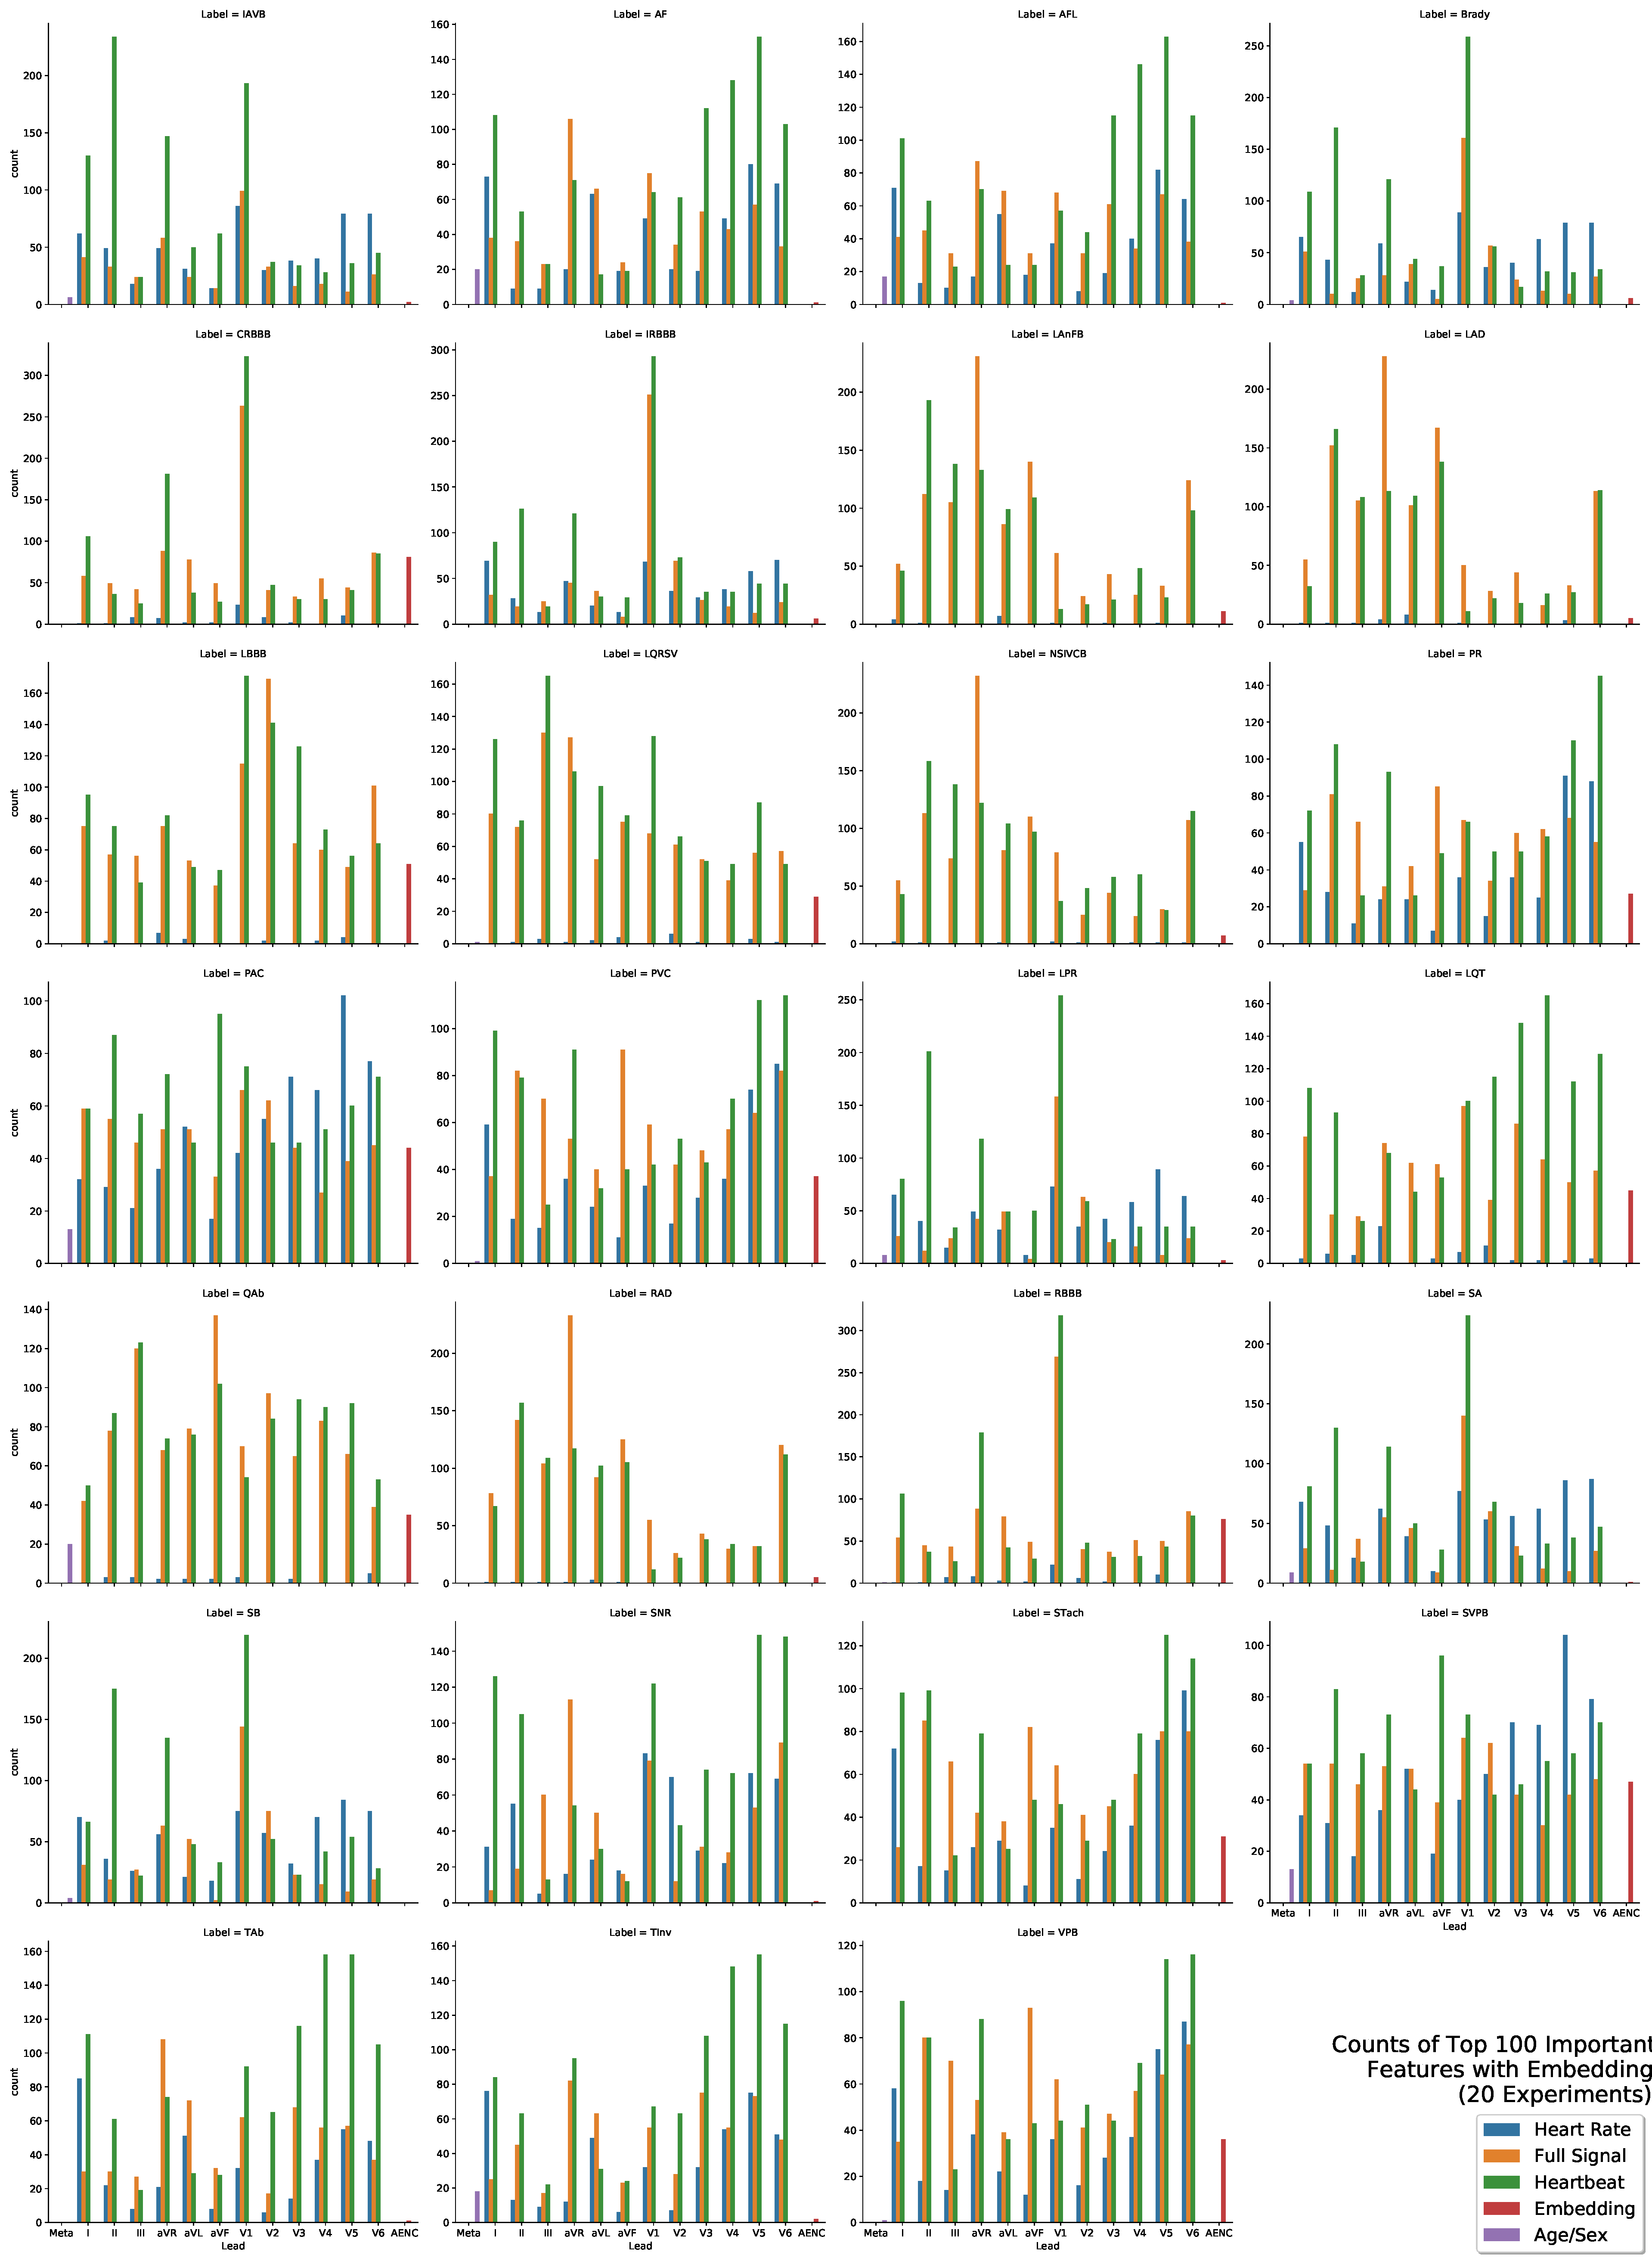
\includegraphics[width=\textwidth]{figure/top_100_feature_importances_all_w_embedding.pdf}
    \caption{Feature importances summary of Configuration~\ref{item:xgb_aenc_model_top_100_w_embd}: ``Top 100 Features with Embeddings", aggregated count over 20 independent experiments. Each of the 27 diagnosed labels displayed separately, showcasing feature derived lead (alternatively Meta or Autoencoder), and category (heart rate, full waveform signal, heartbeat, embedding, age, sex).}
    \label{fig:xgb_aenc_top_100_features_labelwise_count}
\end{figure}

\end{appendices}
\end{document}
